%%%%%%%%%%%%%%%%%%%%%%%%%%%%%%%%%%%%%%%%%
% Beamer Presentation
% LaTeX Template
% Version 1.0 (10/11/12)
%
% This template has been downloaded from:
% http://www.LaTeXTemplates.com
%
% License:
% CC BY-NC-SA 3.0 (http://creativecommons.org/licenses/by-nc-sa/3.0/)
%
%%%%%%%%%%%%%%%%%%%%%%%%%%%%%%%%%%%%%%%%%

%----------------------------------------------------------------------------------------
%	PACKAGES AND THEMES
%----------------------------------------------------------------------------------------

\documentclass{beamer}

\mode<presentation> {

% The Beamer class comes with a number of default slide themes
% which change the colors and layouts of slides. Below this is a list
% of all the themes, uncomment each in turn to see what they look like.

%\usetheme{default}
%\usetheme{AnnArbor}
%\usetheme{Antibes}
%\usetheme{Bergen}
%\usetheme{Berkeley}
%\usetheme{Berlin}
%\usetheme{Boadilla}
%\usetheme{CambridgeUS}
%\usetheme{Copenhagen}
%\usetheme{Darmstadt}
%\usetheme{Dresden}
%\usetheme{Frankfurt}
%\usetheme{Goettingen}
%\usetheme{Hannover}
%\usetheme{Ilmenau}
%\usetheme{JuanLesPins}
%\usetheme{Luebeck}
\usetheme{Madrid}
%\usetheme{Malmoe}
%\usetheme{Marburg}
%\usetheme{Montpellier}
%\usetheme{PaloAlto}
%\usetheme{Pittsburgh}
%\usetheme{Rochester}
%\usetheme{Singapore}
%\usetheme{Szeged}
%\usetheme{Warsaw}

% As well as themes, the Beamer class has a number of color themes
% for any slide theme. Uncomment each of these in turn to see how it
% changes the colors of your current slide theme.

%\usecolortheme{albatross}
%\usecolortheme{beaver}
%\usecolortheme{beetle}
%\usecolortheme{crane}
%\usecolortheme{dolphin}
%\usecolortheme{dove}
%\usecolortheme{fly}
%\usecolortheme{lily}
%\usecolortheme{orchid}
%\usecolortheme{rose}
%\usecolortheme{seagull}
%\usecolortheme{seahorse}
%\usecolortheme{whale}
%\usecolortheme{wolverine}

%\setbeamertemplate{footline} % To remove the footer line in all slides uncomment this line
%\setbeamertemplate{footline}[page number] % To replace the footer line in all slides with a simple slide count uncomment this line

%\setbeamertemplate{navigation symbols}{} % To remove the navigation symbols from the bottom of all slides uncomment this line
}

\usepackage{graphicx} % Allows including images
\usepackage{booktabs} % Allows the use of \toprule, \midrule and \bottomrule in tables
\usepackage{tabularx} % Allows for (middle) vertical centring of the content of table cells
%----------------------------------------------------------------------------------------
%	TITLE PAGE
%----------------------------------------------------------------------------------------

\title[]{8 weeks with CASAL2} % The short title appears at the bottom of every slide, the full title is only on the title page

%\author{Marco Kienzle} % Your name
%\institute[UCLA] % Your institution as it will appear on the bottom of every slide, may be shorthand to save space
%{
%University of California \\ % Your institution for the title page
%\medskip
%\textit{john@smith.com} % Your email address
%}
\date{\today} % Date, can be changed to a custom date

\begin{document}

\begin{frame}
\titlepage % Print the title page as the first slide
\end{frame}

%% \begin{frame}
%% \frametitle{Overview} % Table of contents slide, comment this block out to remove it
%% \tableofcontents % Throughout your presentation, if you choose to use \section{} and \subsection{} commands, these will automatically be printed on this slide as an overview of your presentation
%% \end{frame}

%----------------------------------------------------------------------------------------
%	PRESENTATION SLIDES
%----------------------------------------------------------------------------------------

%% %------------------------------------------------
%% \section{First Section} % Sections can be created in order to organize your presentation into discrete blocks, all sections and subsections are automatically printed in the table of contents as an overview of the talk
%% %------------------------------------------------


%% %------------------------------------------------

\begin{frame}
\frametitle{What is CASAL2?}
\begin{itemize}
\item a C++ software to represent the dynamics of a fishery
\item the dynamics of the fish population is deterministic
\item CASAL2 implements discrete models: it does not have a concept of continuous times (natural mortality are not rates)
\item models are not fitted to catch: catch is an input to the model
\item fishing effort is not used to estimate fishing mortality, instead it uses exploitation rates (U=log(1-F))
\item models can be fitted to abundance surveys, age-frequencies, and more (tagging data, etc..)
\end{itemize}
\end{frame}

%% %------------------------------------------------

\begin{frame}
\frametitle{An approach to learning CASAL2}
Simulating the dynamics of a fishery and feeding CASAL2 with synthetic data, help us:

\begin{itemize}
\item understanding how to use CASAL2 to get the correct parameter estimate
\item learn about the limitations of CASAL2
\end{itemize}

\end{frame}

%%%%%%%%%%%%%%%%%%%%%%%%%%%%%%%%
\begin{frame}
\frametitle{An approach to learning CASAL2}

\begin{figure}
  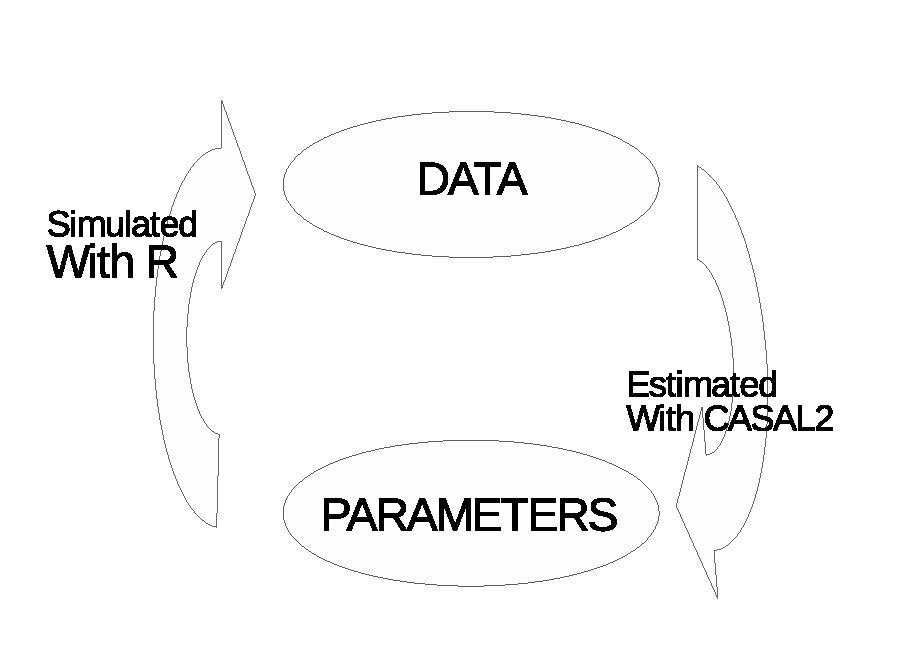
\includegraphics[scale=0.8, angle=0]{diagram.eps}
  \end{figure}

\end{frame}

%% %------------------------------------------------

\begin{frame}
\frametitle{Simulated fishery}

\begin{itemize}
\item Single species, single area
\item age-structured, multiple years
\item number of individuals (no somatic growth)
\item constant: natural mortality, recruitment, selectivity (= 1)
\item varying exploitation rate ($0 \leq U \leq 1$)
\end{itemize}

\end{frame}

%% %------------------------------------------------

\begin{frame}
\frametitle{Synthetic data and parameters passed to CASAL2}

\begin{itemize}
\item catch
\item age frequency distributions
\item abundance survey
\item natural mortality
\item selectivity
\item initial population abundance [sometimes]
\item model structure (timing of the removals, the fraction of natural mortality before remove, etc...) [sometimes]
\end{itemize}

The only thing we are asking to estimate (for the moment) is a single parameter (a constant recruitment): can we estimate that using CASAL2?

\end{frame}

%% %------------------------------------------------


%% %------------------------------------------------

\begin{frame}
\frametitle{Some results}

\begin{table}
  \tiny
\begin{tabular}{|m{4cm}|m{1cm}|m{1cm}|m{4cm}|}
\hline
                & \multicolumn{2}{|c|}{\bf Estimate}                       &          \\ 
  {\bf Simulate}      & {\bf recruitment}          & {\bf Initial conditions} & {\bf Comments} \\ \hline
  Baranov Eq.   & not OK               & not OK                      & you can't implement a Baranov eq. in CASAL2, you need to model a pulse fishery \\ \hline
  Pulse removal & OK                   & not OK                      & CASAL2 assumes un-exploited stock before the start of the data time series \\ \hline
  Pulse removal and virgin stock pre-exploitation & OK & OK          & Finally a CASAL2 model working! I can estimate a single parameter with CASAL2!\\ \hline
\end{tabular}
\end{table}
\end{frame}

%% \subsection{Subsection Example} % A subsection can be created just before a set of slides with a common theme to further break down your presentation into chunks

\begin{frame}
\frametitle{Constant recruitment, variable exploitation rates}

\begin{figure}
  \includegraphics[scale=0.38, angle=-90]{../../TestCASAL2_withSimulatedData/StockDescriptionInNumbers/EstimateSingleConstantRecruitment/ByPassingInitialAbundancesToCASAL2/Results/Graphics/PopDynamics.ps}
  \end{figure}

\end{frame}

%%%%%%%%%%%%%%%%%%%%%%%%%%%%%%%%
\begin{frame}
  \frametitle{Similarity between pulse removal and Baranov}

  We can write that the number at the end of a year is:
  \begin{equation}
    (N_{0} \times e^{-\frac{M}{2}} - N_{c}) \times e^{-\frac{M}{2}}
    \end{equation}

  Since $N_{c} = U \times N_{0} \times e^{-\frac{M}{2}}$, we can rewrite
   \begin{equation}
    N_{0} \times e^{-\frac{M}{2}} (1-U) \times e^{-\frac{M}{2}}
    \end{equation}

   And look at this as
     \begin{equation}
    N_{0} \times e^{-\frac{M}{2}} \times e^{-F} \times e^{-\frac{M}{2}}
     \end{equation}

     So $1-U = e^{-F}$ (Walters and Hilborn, 1992: p.352)
 
  
  \end{frame}


%%%%%%%%%%%%%%%%%%%%%%%%%%%%%%%%
\begin{frame}
\frametitle{Using CASAL2 to estimate constant recruitment}

\begin{figure}
  \includegraphics[scale=0.38, angle=-90]{../../TestCASAL2_withSimulatedData/StockDescriptionInNumbers/EstimateSingleConstantRecruitment/ByPassingInitialAbundancesToCASAL2/Results/Graphics/SimVsEst.ps}
  \end{figure}

\end{frame}

%%%%%%%%%%%%%%%%%%%%%%%%%%%%%%%%
\begin{frame}
\frametitle{Using CASAL2 to estimate constant recruitment}

\begin{figure}
  \includegraphics[scale=0.38, angle=-90]{../../TestCASAL2_withSimulatedData/StockDescriptionInNumbers/EstimateSingleConstantRecruitment/ByPassingInitialAbundancesToCASAL2/Results/Graphics/SimVsEst2.ps}
  \end{figure}

\end{frame}

%%%%%%%%%%%%%%%%%%%%%%%%%%%%%%%%
\begin{frame}
\frametitle{Conclusions}

\begin{itemize}
\item CASAL2 doesn't have (yet) the flexibility to implement any model we want (Baranov equation, delay-difference, survival analysis, etc....)
\item being able to implement only pulse removal fishery is fairly narrow in scope and assuming that a fishery was un-exploited before the start of the data time series is even more limiting
\item we have to do more work to understand why it is failing (in approx 6-10\% of the cases) to converge to the correct recruitment value
\end{itemize}

\end{frame}

%%%%%%%%%%%%%%%%%%%%%%%%%%%%%%%%
\begin{frame}
\frametitle{}

Thanks for your attention

\end{frame}

%% %------------------------------------------------

%% \begin{frame}
%% \frametitle{Blocks of Highlighted Text}
%% \begin{block}{Block 1}
%% Lorem ipsum dolor sit amet, consectetur adipiscing elit. Integer lectus nisl, ultricies in feugiat rutrum, porttitor sit amet augue. Aliquam ut tortor mauris. Sed volutpat ante purus, quis accumsan dolor.
%% \end{block}

%% \begin{block}{Block 2}
%% Pellentesque sed tellus purus. Class aptent taciti sociosqu ad litora torquent per conubia nostra, per inceptos himenaeos. Vestibulum quis magna at risus dictum tempor eu vitae velit.
%% \end{block}

%% \begin{block}{Block 3}
%% Suspendisse tincidunt sagittis gravida. Curabitur condimentum, enim sed venenatis rutrum, ipsum neque consectetur orci, sed blandit justo nisi ac lacus.
%% \end{block}
%% \end{frame}

%% %------------------------------------------------

%% \begin{frame}
%% \frametitle{Multiple Columns}
%% \begin{columns}[c] % The "c" option specifies centered vertical alignment while the "t" option is used for top vertical alignment

%% \column{.45\textwidth} % Left column and width
%% \textbf{Heading}
%% \begin{enumerate}
%% \item Statement
%% \item Explanation
%% \item Example
%% \end{enumerate}

%% \column{.5\textwidth} % Right column and width
%% Lorem ipsum dolor sit amet, consectetur adipiscing elit. Integer lectus nisl, ultricies in feugiat rutrum, porttitor sit amet augue. Aliquam ut tortor mauris. Sed volutpat ante purus, quis accumsan dolor.

%% \end{columns}
%% \end{frame}

%% %------------------------------------------------
%% \section{Second Section}
%% %------------------------------------------------

%% \begin{frame}
%% \frametitle{Table}
%% \begin{table}
%% \begin{tabular}{l l l}
%% \toprule
%% \textbf{Treatments} & \textbf{Response 1} & \textbf{Response 2}\\
%% \midrule
%% Treatment 1 & 0.0003262 & 0.562 \\
%% Treatment 2 & 0.0015681 & 0.910 \\
%% Treatment 3 & 0.0009271 & 0.296 \\
%% \bottomrule
%% \end{tabular}
%% \caption{Table caption}
%% \end{table}
%% \end{frame}

%% %------------------------------------------------

%% \begin{frame}
%% \frametitle{Theorem}
%% \begin{theorem}[Mass--energy equivalence]
%% $E = mc^2$
%% \end{theorem}
%% \end{frame}

%% %------------------------------------------------

%% \begin{frame}[fragile] % Need to use the fragile option when verbatim is used in the slide
%% \frametitle{Verbatim}
%% \begin{example}[Theorem Slide Code]
%% \begin{verbatim}
%% \begin{frame}
%% \frametitle{Theorem}
%% \begin{theorem}[Mass--energy equivalence]
%% $E = mc^2$
%% \end{theorem}
%% \end{frame}\end{verbatim}
%% \end{example}
%% \end{frame}

%% %------------------------------------------------

%% \begin{frame}
%% \frametitle{Figure}
%% Uncomment the code on this slide to include your own image from the same directory as the template .TeX file.
%% %\begin{figure}
%% %\includegraphics[width=0.8\linewidth]{test}
%% %\end{figure}
%% \end{frame}

%% %------------------------------------------------

%% \begin{frame}[fragile] % Need to use the fragile option when verbatim is used in the slide
%% \frametitle{Citation}
%% An example of the \verb|\cite| command to cite within the presentation:\\~

%% This statement requires citation \cite{p1}.
%% \end{frame}

%% %------------------------------------------------

%% \begin{frame}
%% \frametitle{References}
%% \footnotesize{
%% \begin{thebibliography}{99} % Beamer does not support BibTeX so references must be inserted manually as below
%% \bibitem[Smith, 2012]{p1} John Smith (2012)
%% \newblock Title of the publication
%% \newblock \emph{Journal Name} 12(3), 45 -- 678.
%% \end{thebibliography}
%% }
%% \end{frame}

%% %------------------------------------------------

%% \begin{frame}
%% \Huge{\centerline{The End}}
%% \end{frame}

%% %----------------------------------------------------------------------------------------

\end{document} 
